\documentclass[dvips,12pt]{article}

\usepackage[pdftex]{graphicx}
\usepackage{url}
\usepackage{cite}
\usepackage{indentfirst}


\setlength{\oddsidemargin}{0.25in}
\setlength{\textwidth}{6.5in}
\setlength{\topmargin}{0in}
\setlength{\textheight}{8.5in}


% These force using more of the margins that is the default style

\begin{document}

% Everything after this becomes content
% Replace the text between curly brackets with your own

\title{\textbf{Status Versus Utility Classification and Prediction Algorithm for Amazon Products}}
\author{Linda Wogulis, Yijun Zhang}
\date{September 5, 2015}

% You can leave out "date" and it will be added automatically for today
% You can change the "\today" date to any text you like


\maketitle

% This command causes the title to be created in the document

\section{Introduction}

 The main goal for our project is to be able to discern the difference between a product that is being rated or reviewed based on its functionality versus one that is judged for its status. We wish to determine which features of a written review indicate the product'��s utility or status. Results of this research could help improve recommender systems for online products by suggesting a certain type of product based on the user's history of purchases. If a shopper tends to purchase products that are considered ``utility", they should be given more recommendations that are similarly practical, instead of attempting to sell them more frivolous or expensive items. The same can be said for a ``status" shopper, who shouldn't be given the unattractive but practical suggestions. This goal is an attempt at getting a deeper understanding for buyer preferences, and it can improve a system that may not otherwise distinguish between plain black heels that are either \$30 from Forever 21 or \$800 from Gucci.

For our project, we use basic data mining and sentiment analysis techniques in order to produce a model that will predict a product's categorization as either status or utility. We use data from Amazon, and our sample comes from the ``shoes" section of clothing. Our project requires a large quantity of data to be labeled, so we resort to crowdsourcing to do so. We use Amazon Mechanical Turk to obtain workers who label each product on a scale of 1 to 5, with 1 being entirely status and 5 being entirely utility. This data is used to train and test our model, which predicts the status or utility level of new products outside of the original data. 

Plenty of researchers have made similar attempts at representing different aspects of products. Baccianella, Esuli, and Sebastiani'��s \cite{baccianella2009multi} use of vector representation and sentiment analysis mirrors ours - we use bag-of-word features along with linear regression to create a basic model. We take the most commonly occurring words and a few other features of the products - subcategories, price, and number of reviews - and represent them as vectors for each product before solving the linear regression equation. Our model has had success in making predictions about the level of status or utility present in a product.


\section{Related work}

\subsection{Sentiment Analysis}
The past decade has seen a large rise in interest in and research about data mining and sentiment analysis. Bo Pang\cite{pang2008opinion} explains the reasoning behind getting involved in sentiment analysis, which is the widespread demand to know other people's opinions. This can manifest as a desire to sell products and appeal to customers, or it can be as impactful as influencing an election. Pang's research is representative of much of what people have done and are doing related to our project. The central idea is to make accurate predictions of people's opinions based on information from text, whether that be reviews, search engine entries, or one of many other sources of data. Pang's paper describes techniques for determining features of bodies of text. There are many advanced techniques for assigning features to text, and everything described is an option for our model, but we use mainly the bag-of-words system for our project.

\subsection{Aspect-Based Sentiment Analysis}
Our project belongs to a more narrow area called aspect-based sentiment analysis. The goal of basic sentiment analysis is to determine whether something is positive or negative. However, we wish to predict a more specific aspect of the products. Julian McAuley, Jure Leskovec, Dan Jurafsky's 2012 paper ``Learning Attitudes and Attributes from Multi-Aspect Reviews"�� \cite{mcauley2012learning} makes similar use of online reviews. They categorize on the level of sentences, in contrast with our review-level analysis, but the general approach is the same: search for defining features of reviews to predict a more complex concept than positive and negative.  In ``Beyond the Stars: Improving Rating Predictions using Review Text Content" \cite{ganu2009beyond}, authors Gayatree Ganu, Noemie Elhadad, and Amelie Marian argue for the benefit of text-based features as sentiment predictors. We do this with our bag-of-words model, which determines the review-obtained words that are most helpful at predicting a product's category.

\subsection{Crowdsourcing}
Crowdsourcing has been used in many supervised learning tasks. Instead of acquiring very expensive, though reliable, labels from experts, researchers turn to online surveys to collect less accurate labels from multiple workers. Many advances have been made in this new field. 
There are two main concerns with collecting research data through crowdsourcing platforms like Amazon's Mechanical Turk. First, is the data valid and reliable? And second, how do we improve the quality of this data? 
Buhrmester et al. demonstrate that Mechanical Turk workers are more demographically diverse compared to other traditional sampling groups such as standard Internet and college surveys \cite{buhrmester2011amazon}. In addition, several studies show that combining the answers of AMT workers produces result that is of the same quality as domain experts'. 
When attempting to eliminate the effect of spammers on Mechanical Turk, Kittur, Chi and Suh found that adding a verifiable question that takes about the same or less effort than other questions in a survey dramatically decreases suspicious responses \cite{kittur2008crowdsourcing}. In ``Get Another Label? Improving Data Quality and Data Mining Using Multiple, Noisy Labelers"�� Sheng et al. introduce selective repeated-labeling as a tool to improve the overall quality of labels \cite{sheng2008get}.
Based on previous experience and experts'�� suggestions of practices with the best Amazon Mechanical Turk results, we devise a method to collect product labels from the anonymous workers and use them as the input of our regression model.


\section{Approach}

\subsection{Defining the Question}
Before we can build a classifier to distinguish between ``status" and ``utility" goods, we must first develop a precise definition of these concepts.
\subparagraph{Subjective definitions}
We have the option of not explicitly defining the problem, and simply calling it ``status versus utility" when having workers rate products. This allows for individuals' opinions to contribute, and hopefully a universal idea on what these terms mean is apparent. However, this system is not extremely reliable because it makes an unjustifiable assumption - that all responders have an inherent understanding of what status and utility goods are. 
\subparagraph{Objective definitions}
What we are calling a ``status good"�� is frequently called a ``Veblen good" in the economics world. The definition states that a Veblen good is one ``for which demand increases as the price increases, because of its exclusive nature and appeal as a status symbol"�� \cite{veblen}. This definition may be possible to model mathematically, but we find that a basic regression using the features of price and popularity yields a model with no significant correlations for either feature. The precise mathematical definition of the desired label does not seem to aid in creating a base of labels with which to train a model.
\subparagraph{Guided subjective definitions}
What matters is to create a predictor that will model a real aspect of the product that affects buyers' choices. So, a definition that doesn't restrict a rater's innate sense of the terms'�� meanings while still explaining the overall concept is ideal. Raters are therefore told that a utility good is one that is bought mainly because of its functionality, effectiveness, or usefulness, while a status good is one that is bought with the aim of increasing one's social desirability, or because the buyer sees the object as something attractive or desirable regardless of their need for the product'��s functional use. The wording accounts for Veblen goods, which are desired more than they should be, considering their price, which would otherwise be based on the product's utility. This definition requires the rater to recognize which products are seen in what light, and to have a basic knowledge of society's beauty standards and current fashions. Although this method depends on unreliable raters'�� accuracy, it manages to present the question in the most precise way possible while allowing for individuals' natural understanding of the concept to show through, ultimately 

\subsection{Selecting Workers}
To see whether people generally agree on categorizing products between ``��status goods" and ``utility goods"��, we use Amazon's Mechanical Turk (AMT) to ask our subjects to
collectively label 2000 Amazon products. AMT is an online labor market that allows one to outsource small tasks (Human Intelligence Tasks, or HITs) to a large pool of workers for relatively low pay, and it has been used extensively for a variety of research topics. The main drawback to using AMT is the difficulty obtaining high quality data, especially avoiding spammers who attempt to make money without honestly answering the questions. There are two things we do to reduce the noise caused by apathetic workers:

\subparagraph{Qualification}
A HIT approval rate indicates what percentage of the worker's responses are accepted by requesters. We assign our task to the workers only if they have already completed over 500 HITs and their HIT approval rate is above 95\%. In addition, we include a captcha question asking them to describe any aspect about the products that helped them make their decisions. Not having a reasonable answer to this question can result in their HIT being rejected.

\subparagraph{Repeated Labeling}
Previous work has shown that repeated-labeling, the process of having multiple individuals labeling some or all of the data points, directly improves the quality of labeled data \cite{sheng2008get}. We tested our labeling task on a small product sample and decided that five labelers produce the most cost-efficient result for our purposes.

\subsection{Cleaning up Data}

\subparagraph{Worker reliability} \label{reliability}
Once we collect the data from Amazon Mechanical Turk, we have to determine the reliability of the workers. We look through responses to attempt to eliminate any obviously computer-generated or uncaring answers. However, this proves more difficult than expected. We wish to eliminate suspicious answers, but the only suspicious responses are when the worker assigns every product the same number. We do not find any instances of this, so we must calculate which workers' answers are not in line with the majority - that is, which workers appear to have no correlation between their ratings and those of the other workers. To do this, we choose to calculate the Pearson correlation coefficient, r, for each pair of workers that rated any common products. Pearson's r is a value between -1 and 1 that indicates the similarity between two sets of numbers. -1 signifies perfect negative correlation, 0 is no correlation (equivalent to random), and 1 is perfect positive correlation. The Pearson correlation coefficient is ideal for our purposes because it takes into account how far away values are given the scale, instead of simply counting whether or not they are equal, as other methods do.

After calculating each worker's Pearson correlation coefficient in relation to others' ratings, we take the workers who have a negative average correlation and remove them from the dataset. This eliminates the least reliable workers. There are only three workers with negative correlations in our dataset, and each worker only rated 10 or 20 products, so there is little effect on the model. However, after the elimination of the negative valued workers, the correlation values for the other workers all either increase a small amount or remain the same. The initial average Pearson's correlation value was .316, and after removing the three workers' responses, it increases to .339, a difference of .023. This is clearly an improvement, but we don't know quite how much of one. In order to determine how significant this change is, we would have to compute the r-squared values for the dataset both with the negative-valued workers and without them. 

\begin{figure}[h]
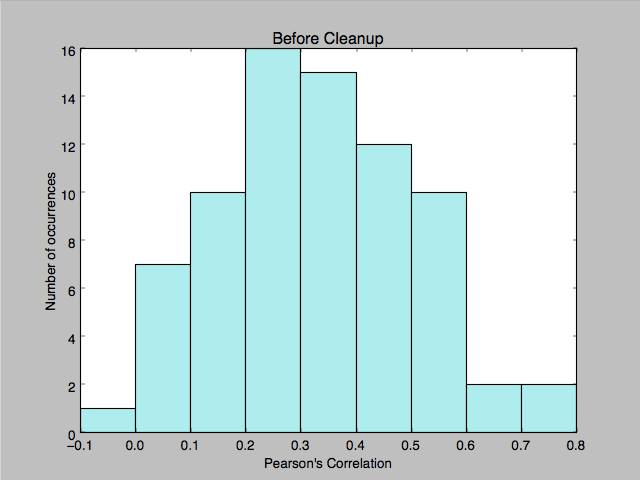
\includegraphics[scale=0.36]{hist_bad}
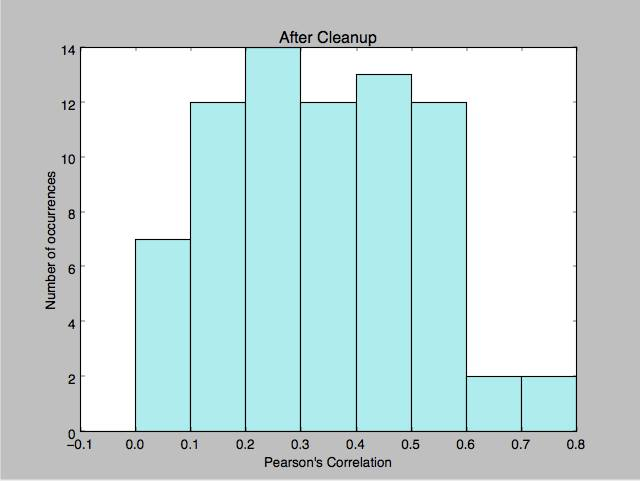
\includegraphics[scale=0.36]{hist_good}
\caption{Histograms of the Pearson correlations before removing the workers with negative values (left) and after doing so (right)}
\end{figure}

\subparagraph{Deciding on a label}
Despite the level of similarity between the raters, very few groups of labels are consistent. So, we must devise a method to determine what label we will use for the product in question. There are five possible numbers for raters to choose. It seems reasonable that if three people pick the same number, it is a reliable value, considering how rarely it happens. So, we will use it as our final label. Because this is not extremely common, even for products with clear and consistent labels, we must have a second way of assigning a valid label. If one rater is unreliable, but the rest are grouped similarly, we want to avoid skewing the label away from its true value. So, if four or more of the raters fall on one side of the scale (3 being the middle, or average, value, and it is inclusive), we take the average of the numbers that are included in said group. For example, if the ratings are: 3, 1, 1, 5, and 2; the final label with be calculated as the average between 3, 1, 1, and 2, or (3+1+1+2)/4=1.75. If the labels fit neither criteria, we do not have a system we trust to obtain an accurate label, so we omit it from our data.

\subsection{Modeling}

\subparagraph{The Naive Model}

We first use the labeled data obtained from AMT to build a linear regression-generated model. The basic idea of linear regression is to use the equation $Ax=b$, with each variable being a matrix. $A$ is a matrix of feature vectors, $x$ is the multiplication factor to be solved for, and $b$ is the resulting value to be predicted. For our project, $b$ is the place along the spectrum of status and utility, on a scale of 1 to 5, with 1 being entirely status and 5 being entirely utility. $A$ consists of feature vectors from product reviews. Each row of $A$ contains a product's relevant information, organized in columns corresponding to features such as its bag-of-words representation or its price. We solve the regression equation to find $x$ by training on a dataset and trying different feature vectors in $A$.
An outlier like a rare but very strongly emotional word can cause undesirable behavior in our model. If a review containing an outlier happens to correspond to products that have extreme labels (1 or 5), the rare word might have a very large coefficient that may not be effectively predictive of new data.

\subparagraph{Ridge Regression}
In response to the overfitting problem of linear regression, we apply ridge regression. Instead of using $|| y - X * \theta ||$ to compute the error, ridge regression introduces the term $\lambda * \theta$ to regularize features, so that the extremely large coefficients are penalized. Therefore, outliers in the data have less effect on the coefficients. We run several trials using validation dataset to fit the model and choose the parameter $\lambda$ that gives the lowest sum of squared error. 

\section{Evaluation/Results}

\subsection{Can people agree upon what it means for a product to be a ``status good"�� or a ``��utility good"?}
Addressing this question is a necessary precursor to the overall project because we must have a stable definition for what is is we're trying to categorize. If there is no universal understanding of a difference between the two categories, our model will have nothing meaningful to predict. 

We use Amazon'��s Mechanical Turk to ask our subjects to collectively label Amazon product data, so we must ensure that the labeling we receive is accurate. To do this, we calculate the Pearson correlation coefficients between each worker, between two ``ideal"�� workers (the researchers), and between the two ideal workers and the Mechanical Turk workers. 

The correlations within the Mechanical Turk workers were briefly discussed above, in \ref{reliability}. To start, the average Pearson correlation for the workers who are used in the final model is .339. This shows that there is at least some aspect of the products that indicates ``��status" or �``utility" to a large portion of responders. Only three workers (of 77 total) had negative values originally, and they were all above -.19. There were also five workers with values of 0, which remain at 0 after removing the three with negative correlations. So, almost 90\% of the workers had Pearson correlation coefficients greater than 0. 

To understand what this says about the quality of Mechanical Turk workers, we first compare to the correlation between the two ideal workers, which was found to be .503. This is reasonably higher than that among the workers, which is expected. We have determined that the correlation between the two ideal workers is the highest Pearson's r possible, since they are the best available workers. Knowing this, and understanding that the workers are not expected to achieve that high of an average, we see that a .339 average is reasonable. The workers'�� correlations are lower than ideal, but they are still significantly above zero, so they fall right where we expect and desire them.

To obtain the correlations between each ideal worker and the Mechanical Turk workers, we sample the HITs and compare our answers to randomly selected workers' answers. Taking a sample allows us to rate a small number of products and still obtain a representative sample through randomization.
As we hoped, the correlations between each ideal worker and a random sampling of the group of Mechanical Turk workers are both between the aforementioned average correlations of .339 and .503, landing at .416 and .477. These end up being next to each other in the ordered list of workers' correlations, enforcing the assumption that the two ideal workers are similarly ideal. 

From this, we can see that it is reasonable to say that strangers  can, for the most part, agree upon what it means for a product to be a ``status good" or a ``utility good". We have enough confidence in our ability to accurately label products based on Mechanical Turk workers' input that we can proceed with the second question in our project.

\begin{table}[h]
	\centering
	\label{my-label}
	\begin{tabular}{lllll}
		\cline{1-3}
		\multicolumn{1}{|l|}{Pearsons Correlations}   & \multicolumn{1}{l|}{Ideal Worker 1}          & \multicolumn{1}{l|}{Mechanical Turk Workers} &  &  \\ \cline{1-3}
		\multicolumn{1}{|l|}{Ideal Worker 2}          & \multicolumn{1}{l|}{0.503006380153}          & \multicolumn{1}{l|}{0.416399099835 (sample)} &  &  \\ \cline{1-3}
		\multicolumn{1}{|l|}{Mechanical Turk Workers} & \multicolumn{1}{l|}{0.477211356069 (sample)} & \multicolumn{1}{l|}{0.339485946 (average)}   &  &  \\ \cline{1-3}
	\end{tabular}
	\caption{Workers' Quality Comparison}
\end{table}

\subsection{Can we train a model to predict the categorization of each product as status or utility? }


The r-squared score is a standard measure of how close a fitted model is to the real data. In 5 trials we run, our model manages to get an average r-squared score of 0.4054. Given that the Pearsons Correlation between two ideal workers is 0.5030, which means there are natural disagreement among people which make some products controverial and hard to predict, we shall not disapprove our second hypothesis.


Figure 2 shows the prediction result of 200 products in a training dataset. It turns out that our model does a better job at predicting utility goods.

\begin{figure}[h] \label{scatterplot}
	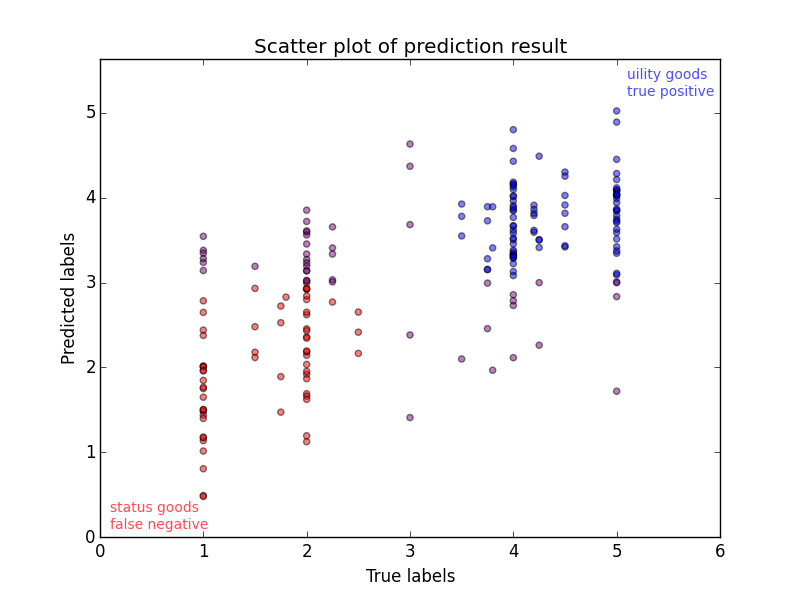
\includegraphics[scale=0.6]{scatter}
	\centering
	\caption{A scatter plot of 200 products with their true labels and predicted labels. The true labels are on the x-axis and the predicted labels are on the y-axis.}
\end{figure}

Table 2 describes the performance of our model. It has 89.80\% accuracy when predicting utility products, and 54.36\% accuracy when predicting status products.


\begin{table}[h]
	\centering
	\begin{tabular}{lllll}
		\cline{1-3}
		\multicolumn{1}{|l|}{True/Predicted labels} & \multicolumn{1}{l|}{Utility} & \multicolumn{1}{l|}{Status}  &  &  \\ \cline{1-3}
		\multicolumn{1}{|l|}{Utility}               & \multicolumn{1}{l|}{89.80\%} & \multicolumn{1}{l|}{10.20\%} &  &  \\ \cline{1-3}
		\multicolumn{1}{|l|}{Status}                & \multicolumn{1}{l|}{45.74\%} & \multicolumn{1}{l|}{54.36\%} &  &  \\ \cline{1-3}                                  
	\end{tabular}
	\caption{Classification Performance of the Model}
\end{table}


Figure 3 shows the most indicative 30 words people use when reviewing utility and status products. 

\begin{figure}[h]
	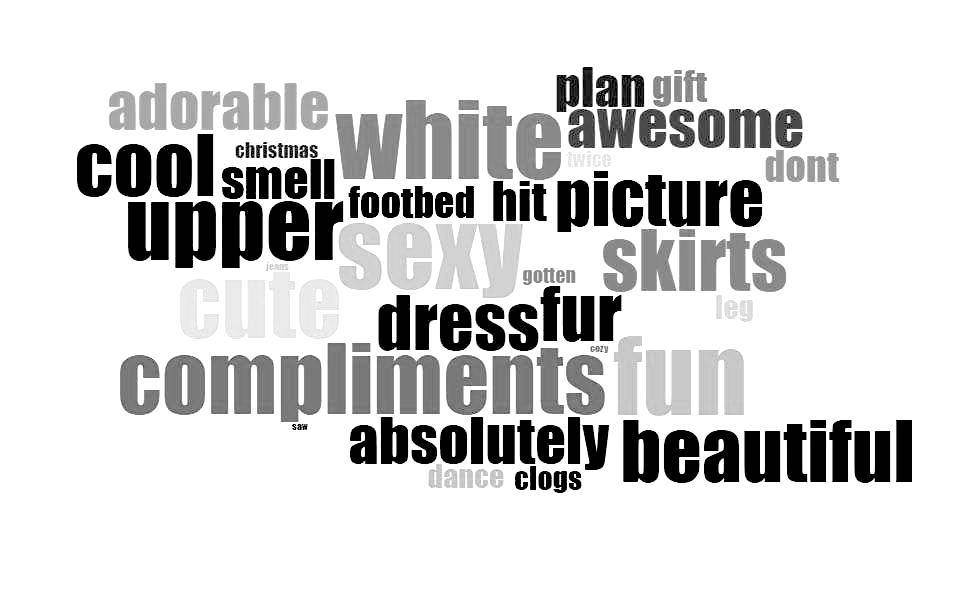
\includegraphics[scale=0.245]{Status_bw}
	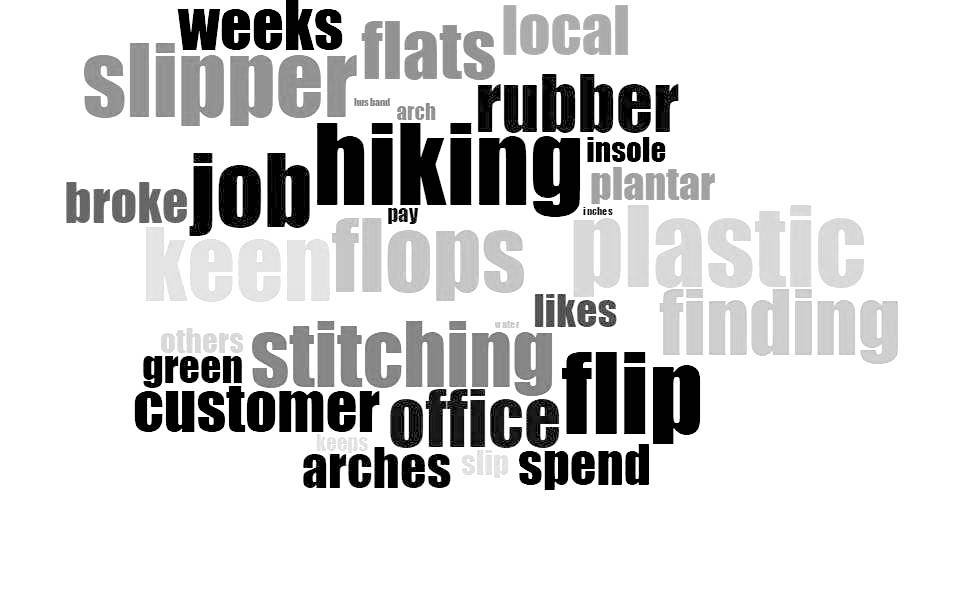
\includegraphics[scale=0.245]{Utility_bw}
	\caption{Word-cloud visualization of most indicative words people use when reviewing status (left) and utility (right) products}
\end{figure}

Inevitably, people mention brands in their reviews. So, we have separated the brand names from the ranking result and list as below:
\\
\\
\noindent Brands associated with...

\noindent Utility products: Crocs, Velcro, Saucony, Clarks

\noindent Status products: Birkenstock, Dansko



\section{Discussion}

Our true labels are not perfect, and so we expect the predictor to have a lower ceiling on accuracy. Considering this, our results suggest that we have a model that predicts a product's labeling as either status or utility with a significant level of accuracy - our model predicts the correct label 73\% of the time. We found that there is a shared sense of what status goods and utility goods are, and that it is possible to build a predictor for this classification based on text mining of Amazon reviews.

The main improvement to be made to our research is to experiment with different features. We stuck with the price, popularity, subcategory, and most significant words in the reviews. Adding new features, such as the length of the review or the brand name, could improve the model. Varying which features are used in conjunction with each other could also affect the accuracy of the model. Because our accuracy depends on the accuracy of our original, true labels, it may also be beneficial to devise a more intricate and reliable method for selecting labels from Mechanical Turk results. In terms of overall structure, the project could alternately be designed as a semi-supervised model in order to allow a smaller set of original data. This could result in a more accurate model because the original labels would be more reliable, as we would be able to take a smaller set to start.


\bibliography{document}{}
\bibliographystyle{plain}



\end{document}
